\section{Results} %5.4
\subsection{Results and Analysis} %5.4.1
\label{subsection5.4.1}

All the acceptable points can be seen as Figure~

\begin{figure}[htbp]
\centering
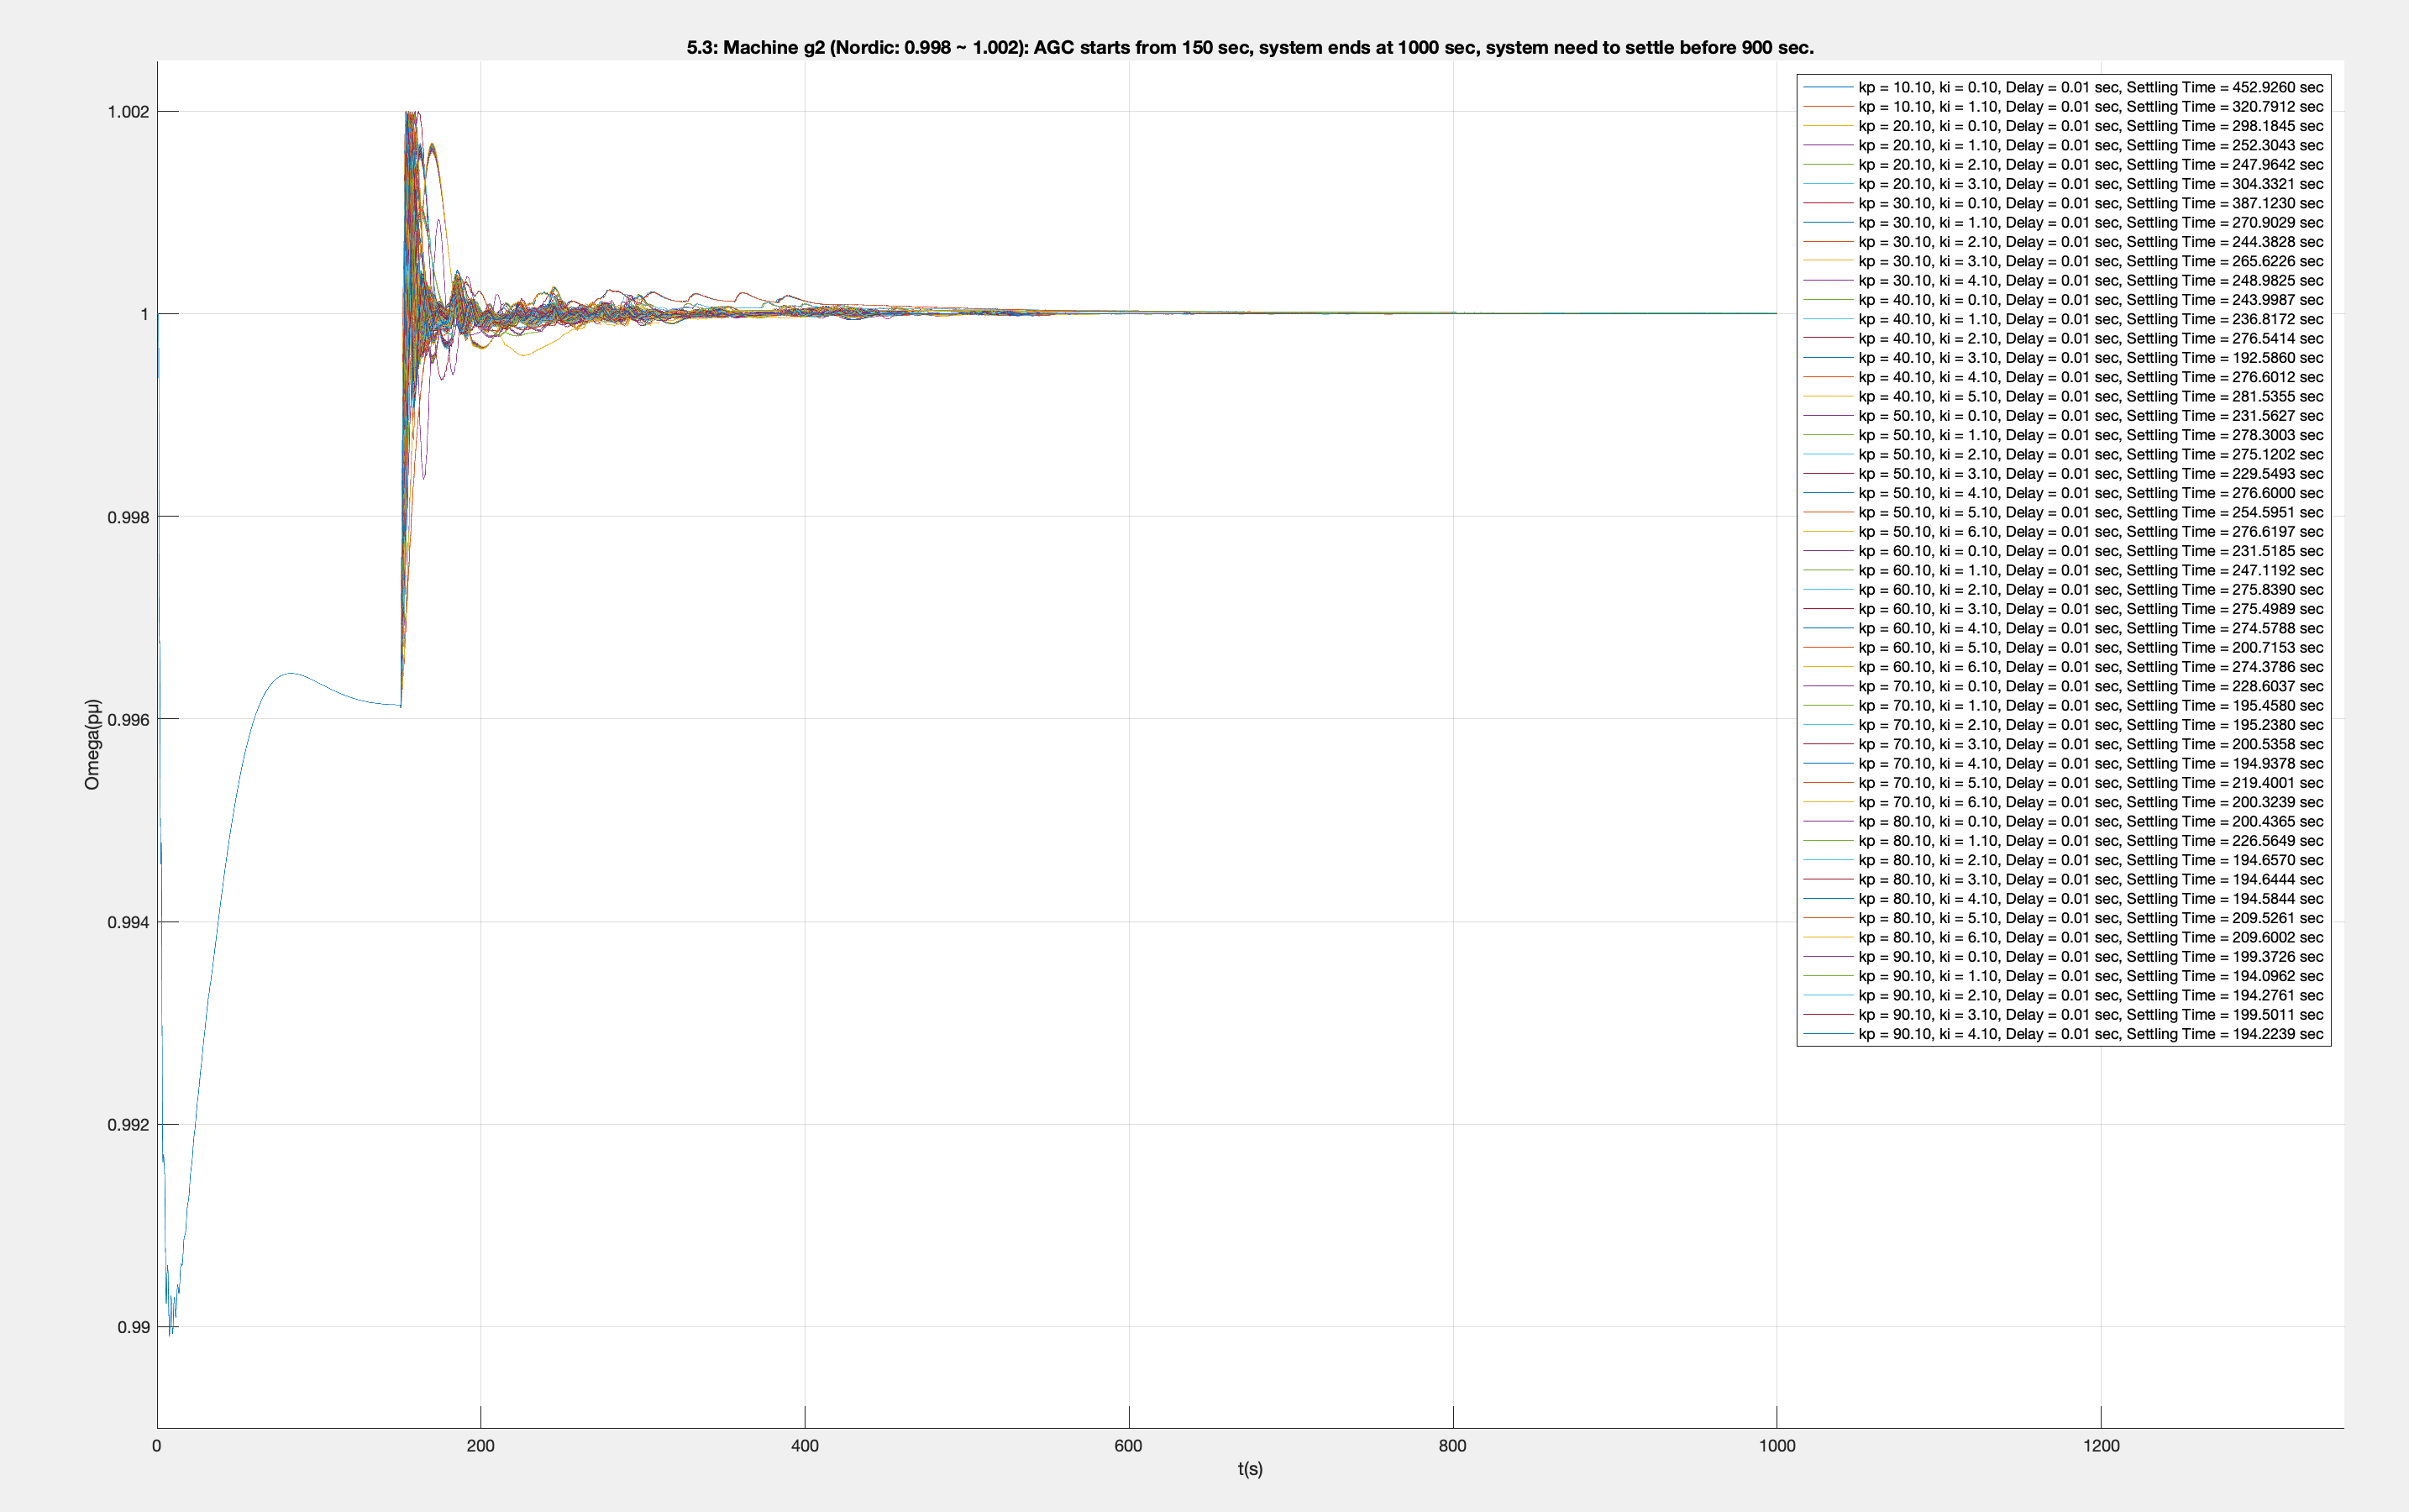
\includegraphics[width = .819\textwidth]{figure/5_4_1_i.png}
\caption{Impact of time delay: all the acceptable points}
\label{5_4_1_i}
\end{figure}


The final 3D Triangle Surface plot shows in Figure~\ref{5_4_1_Outlier}. 

\begin{figure}[htbp]
\centering
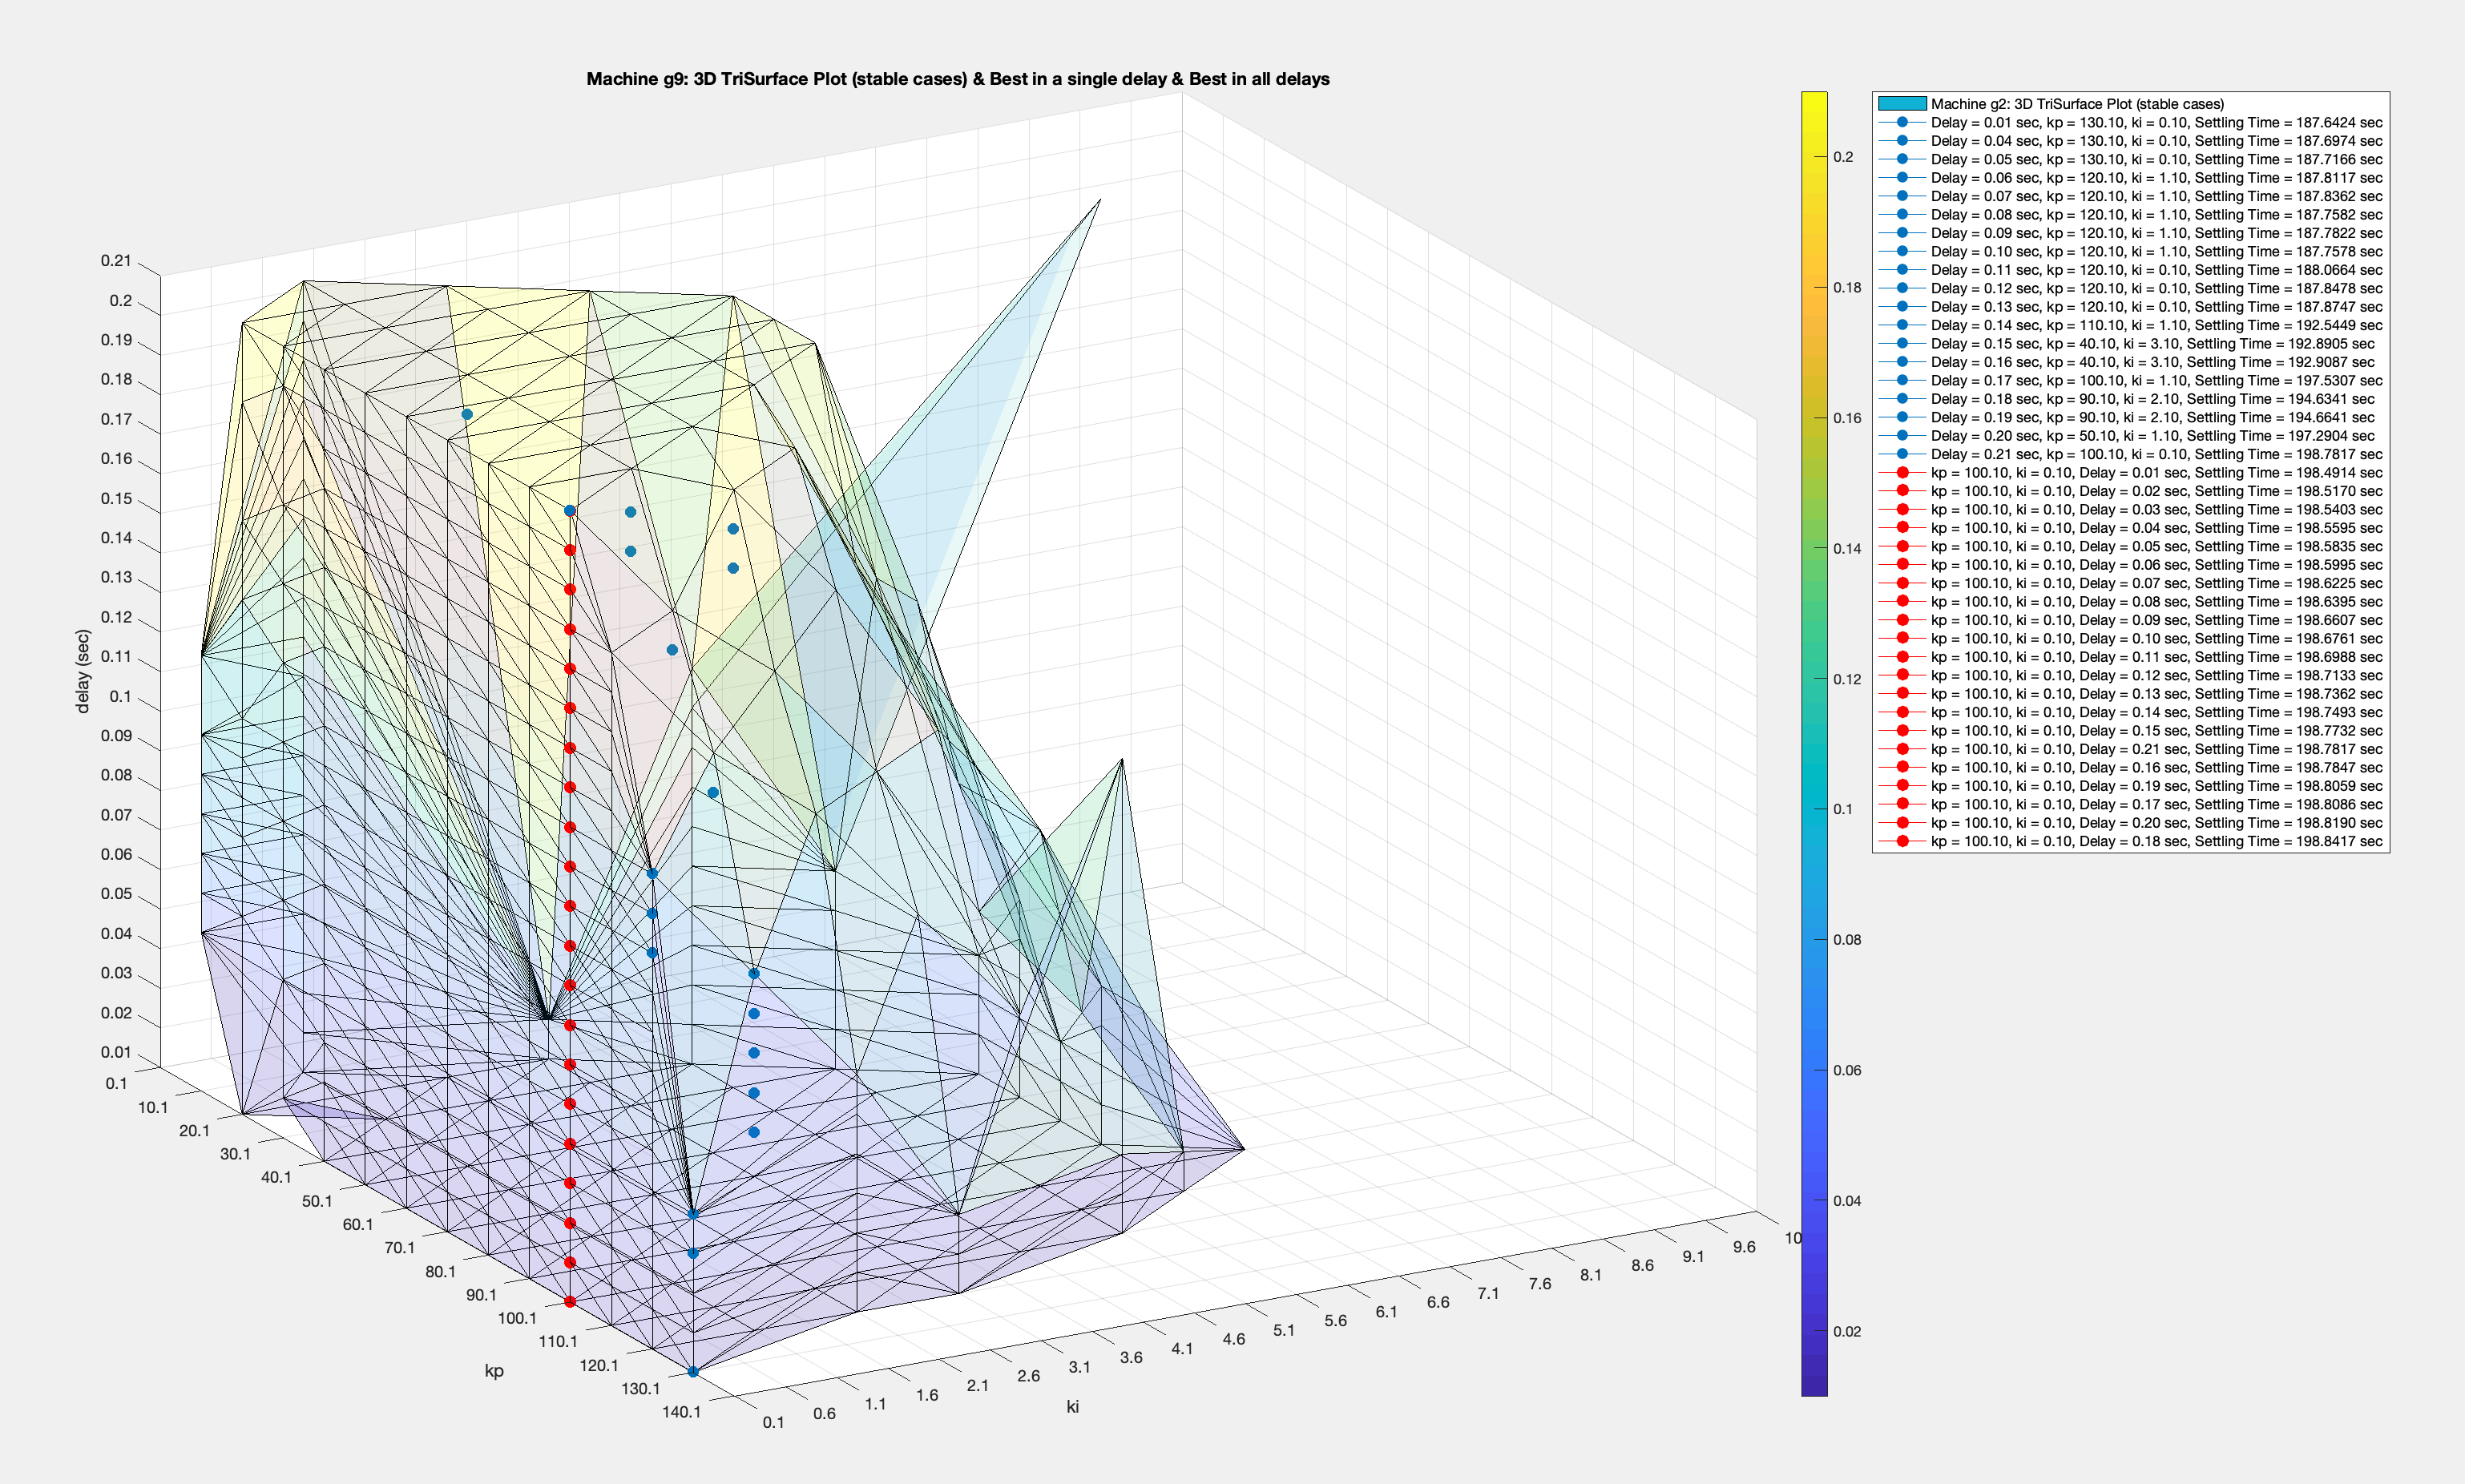
\includegraphics[width = .819\textwidth]{figure/5_4_1_Outlier.png}
\caption{3D plot: contain outliers}
\label{5_4_1_Outlier}
\end{figure}

From Figure~\ref{5_4_1_Outlier}, we can see that there are some outliers here. These outliers can be seen as part of the acceptable results. However, in reality, these outliers can be seen as interference data that we can remove them for a better analysis.\\

\begin{figure}[htbp]
\centering
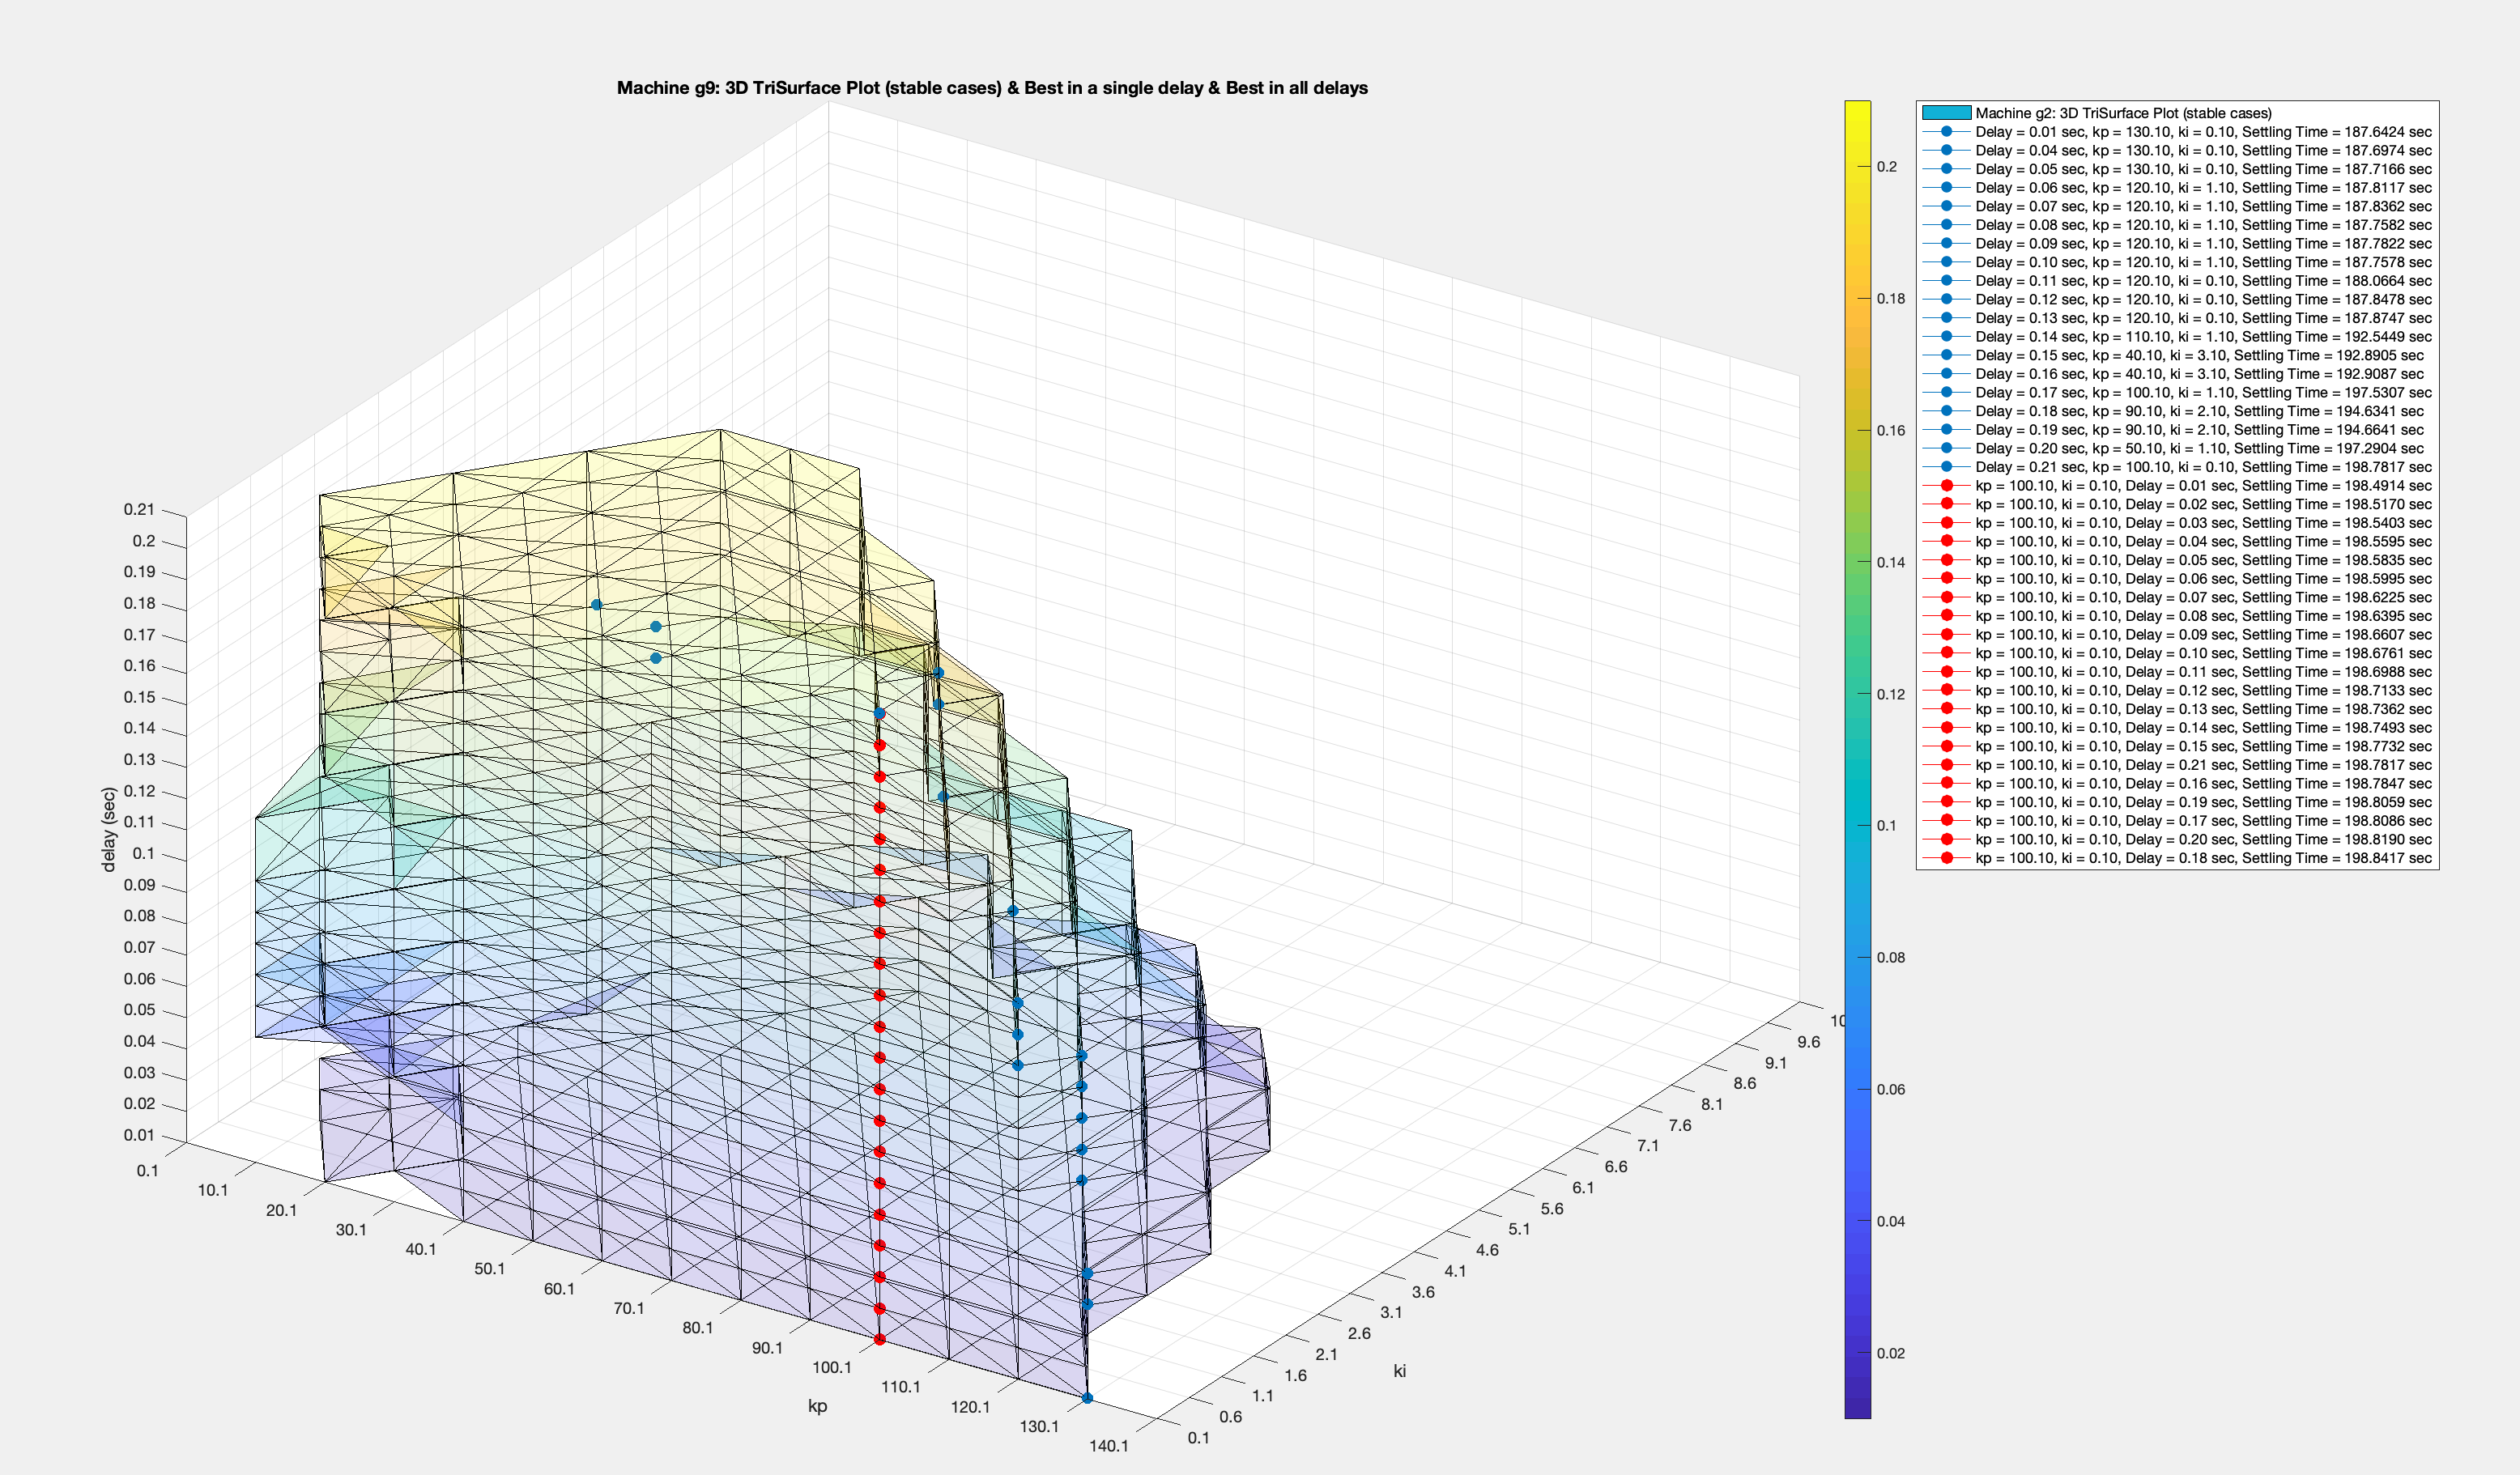
\includegraphics[width = .819\textwidth]{figure/5_4_1_without_Outlier1.png}
\caption{3D plot front side: without outliers}
\label{5_4_1_without_Outlier1}
\end{figure}

\begin{figure}[htbp]
\centering
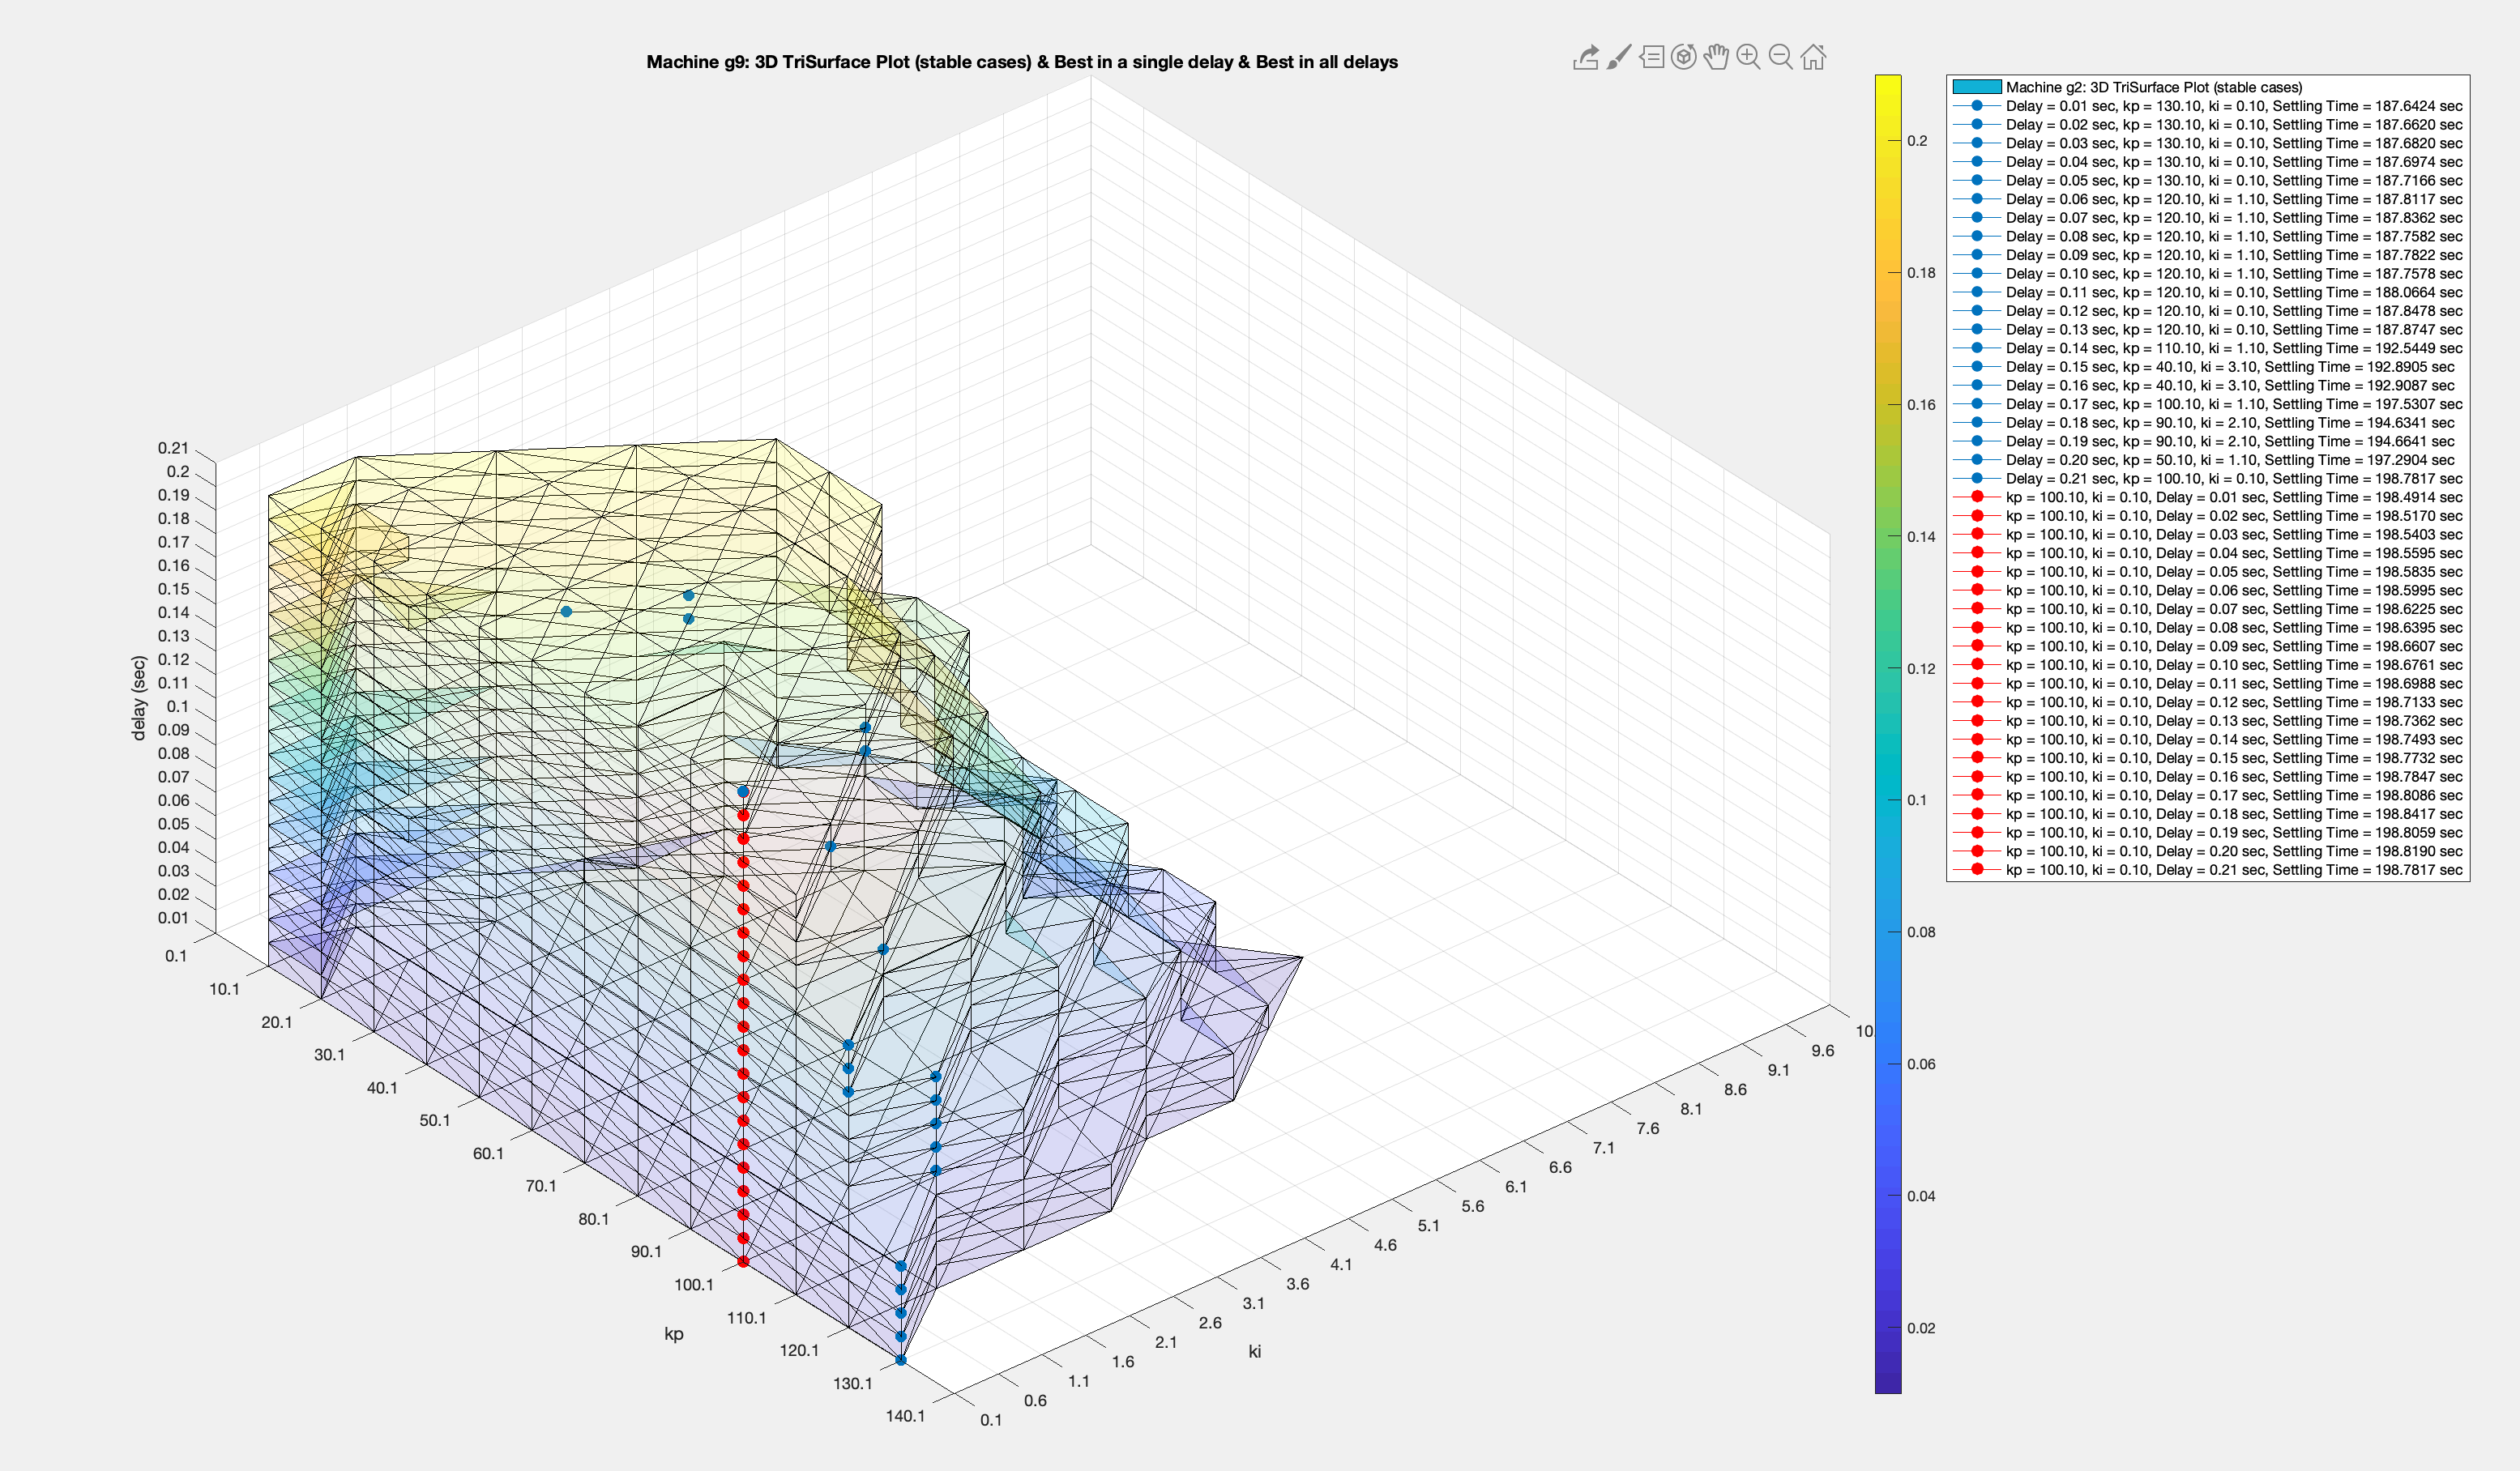
\includegraphics[width = .819\textwidth]{figure/5_4_1_without_Outlier2.png}
\caption{3D plot right side: without outliers}
\label{5_4_1_without_Outlier2}
\end{figure}


\begin{figure}[htbp]
\centering
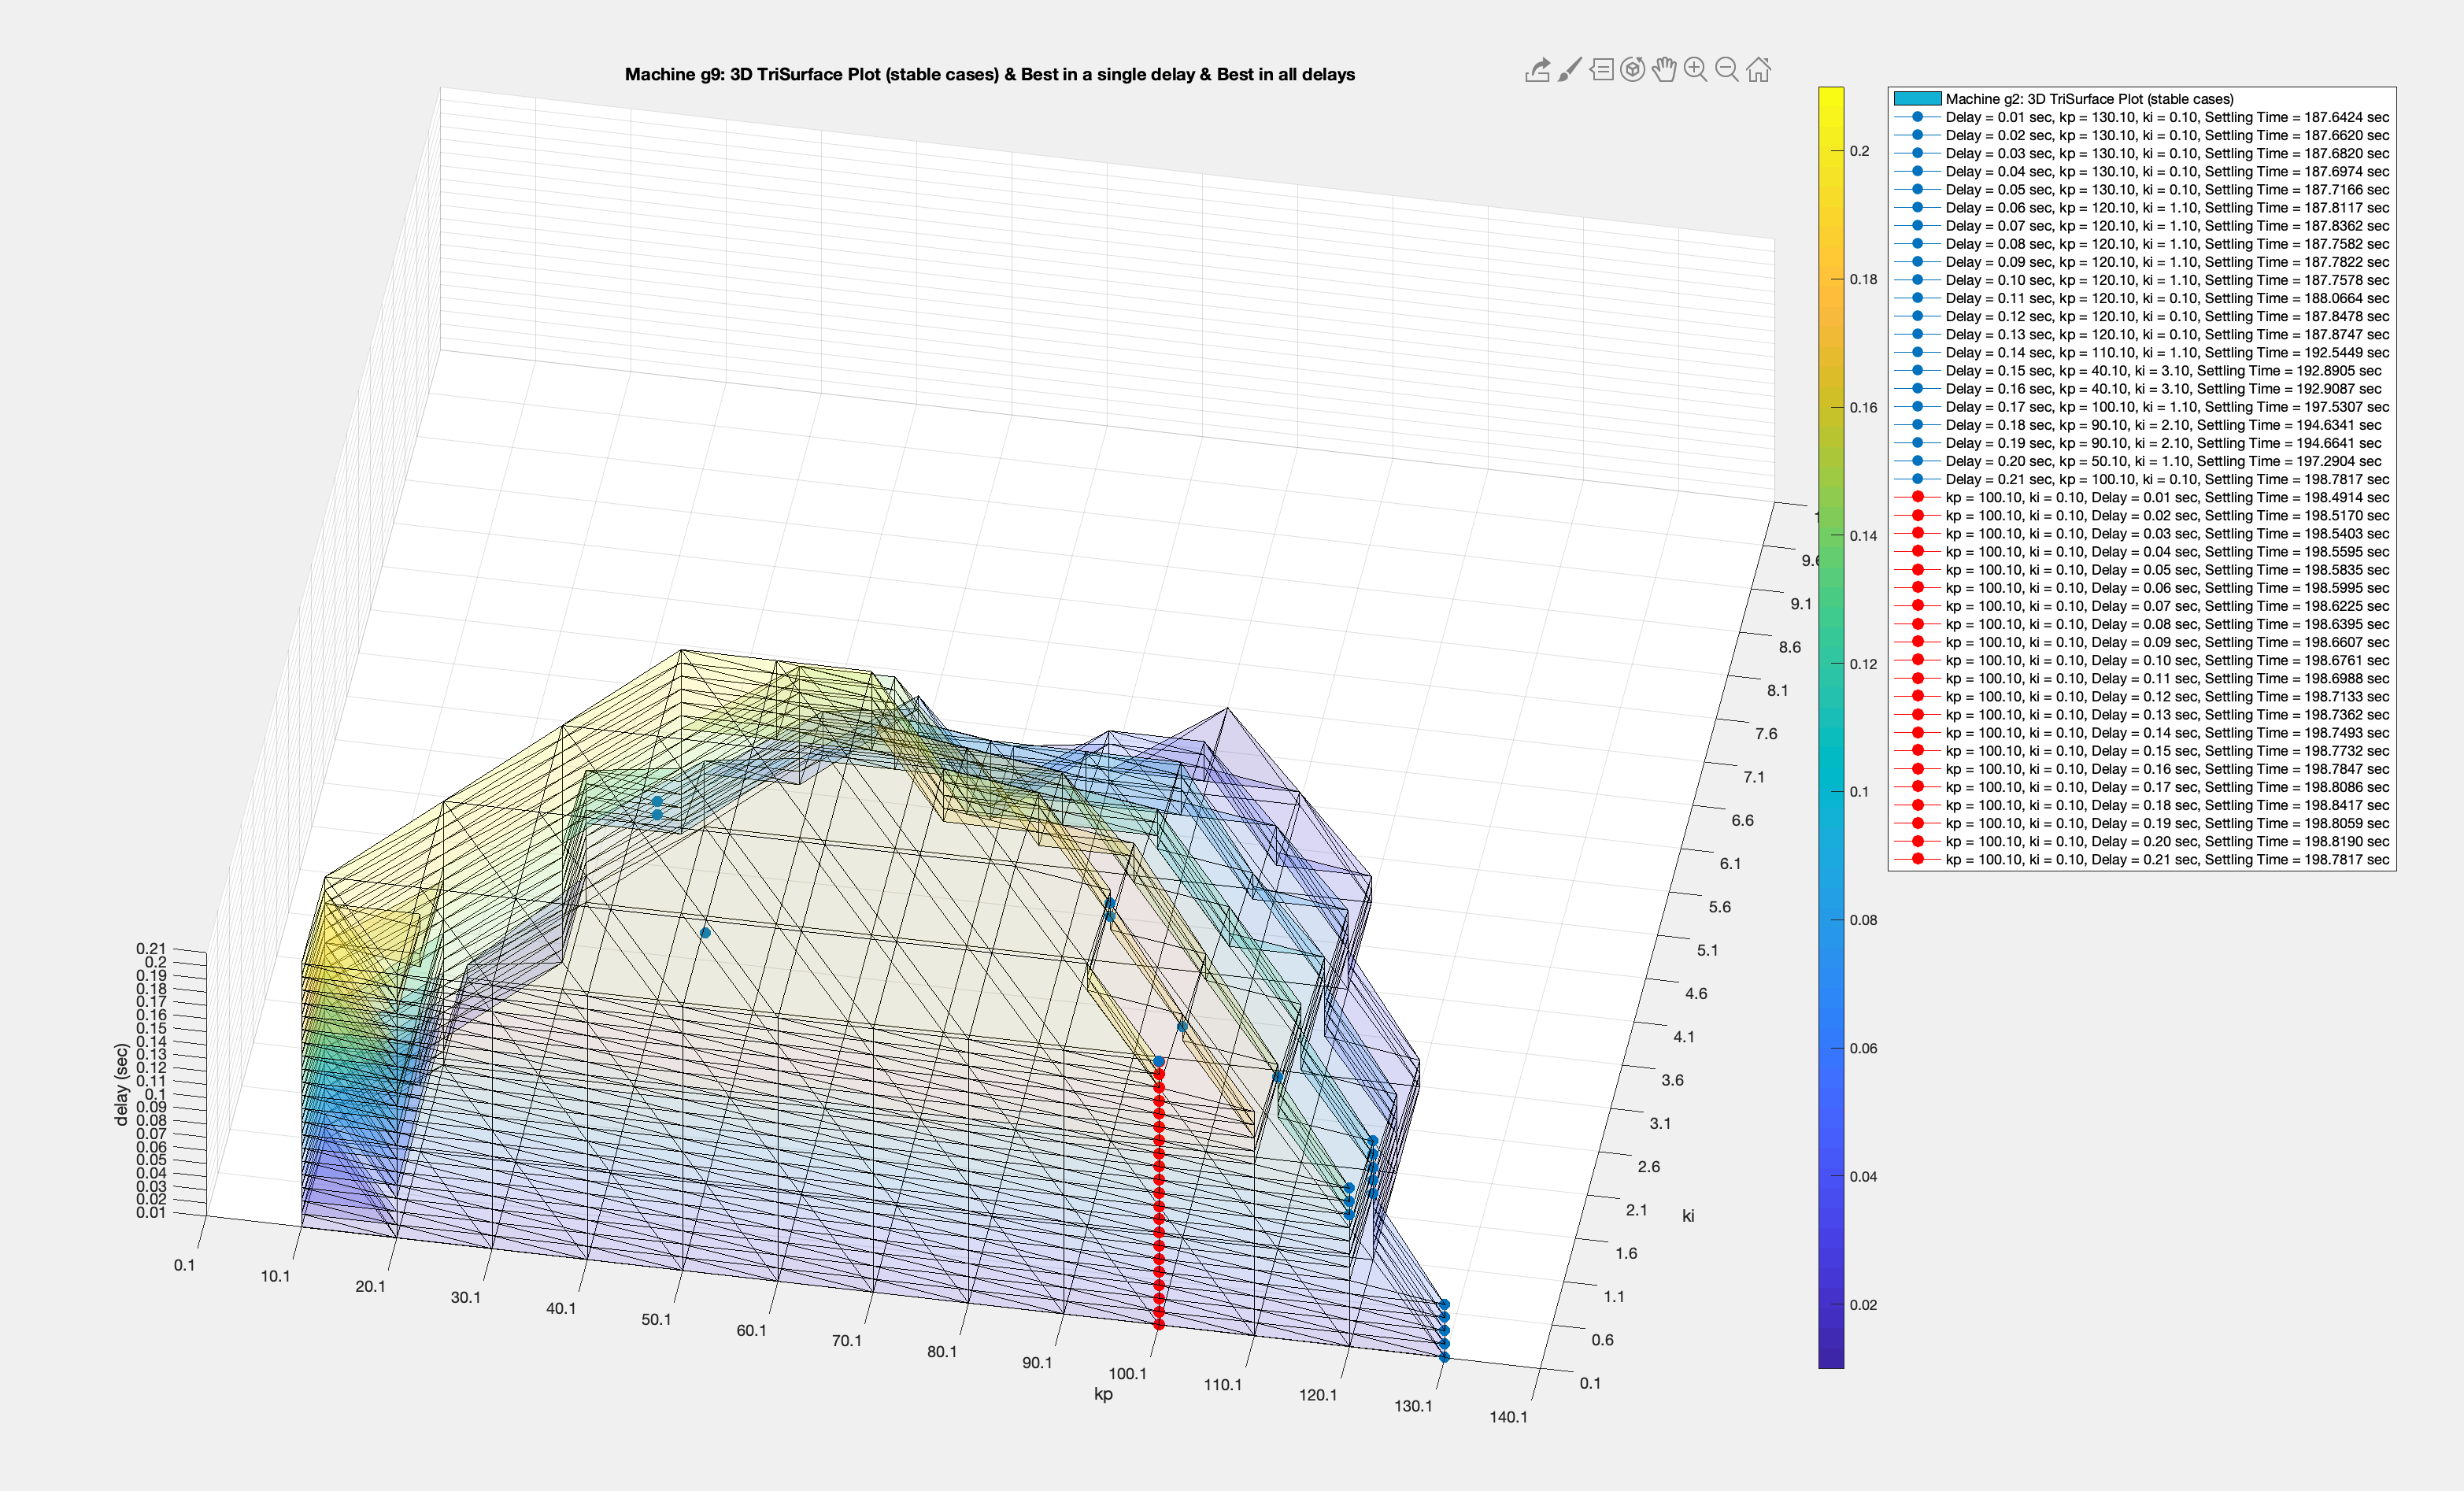
\includegraphics[width = .819\textwidth]{figure/5_4_1_without_Outlier3.png}
\caption{3D plot top side: without outliers}
\label{5_4_1_without_Outlier3}
\end{figure}


\begin{figure}[htbp]
\centering
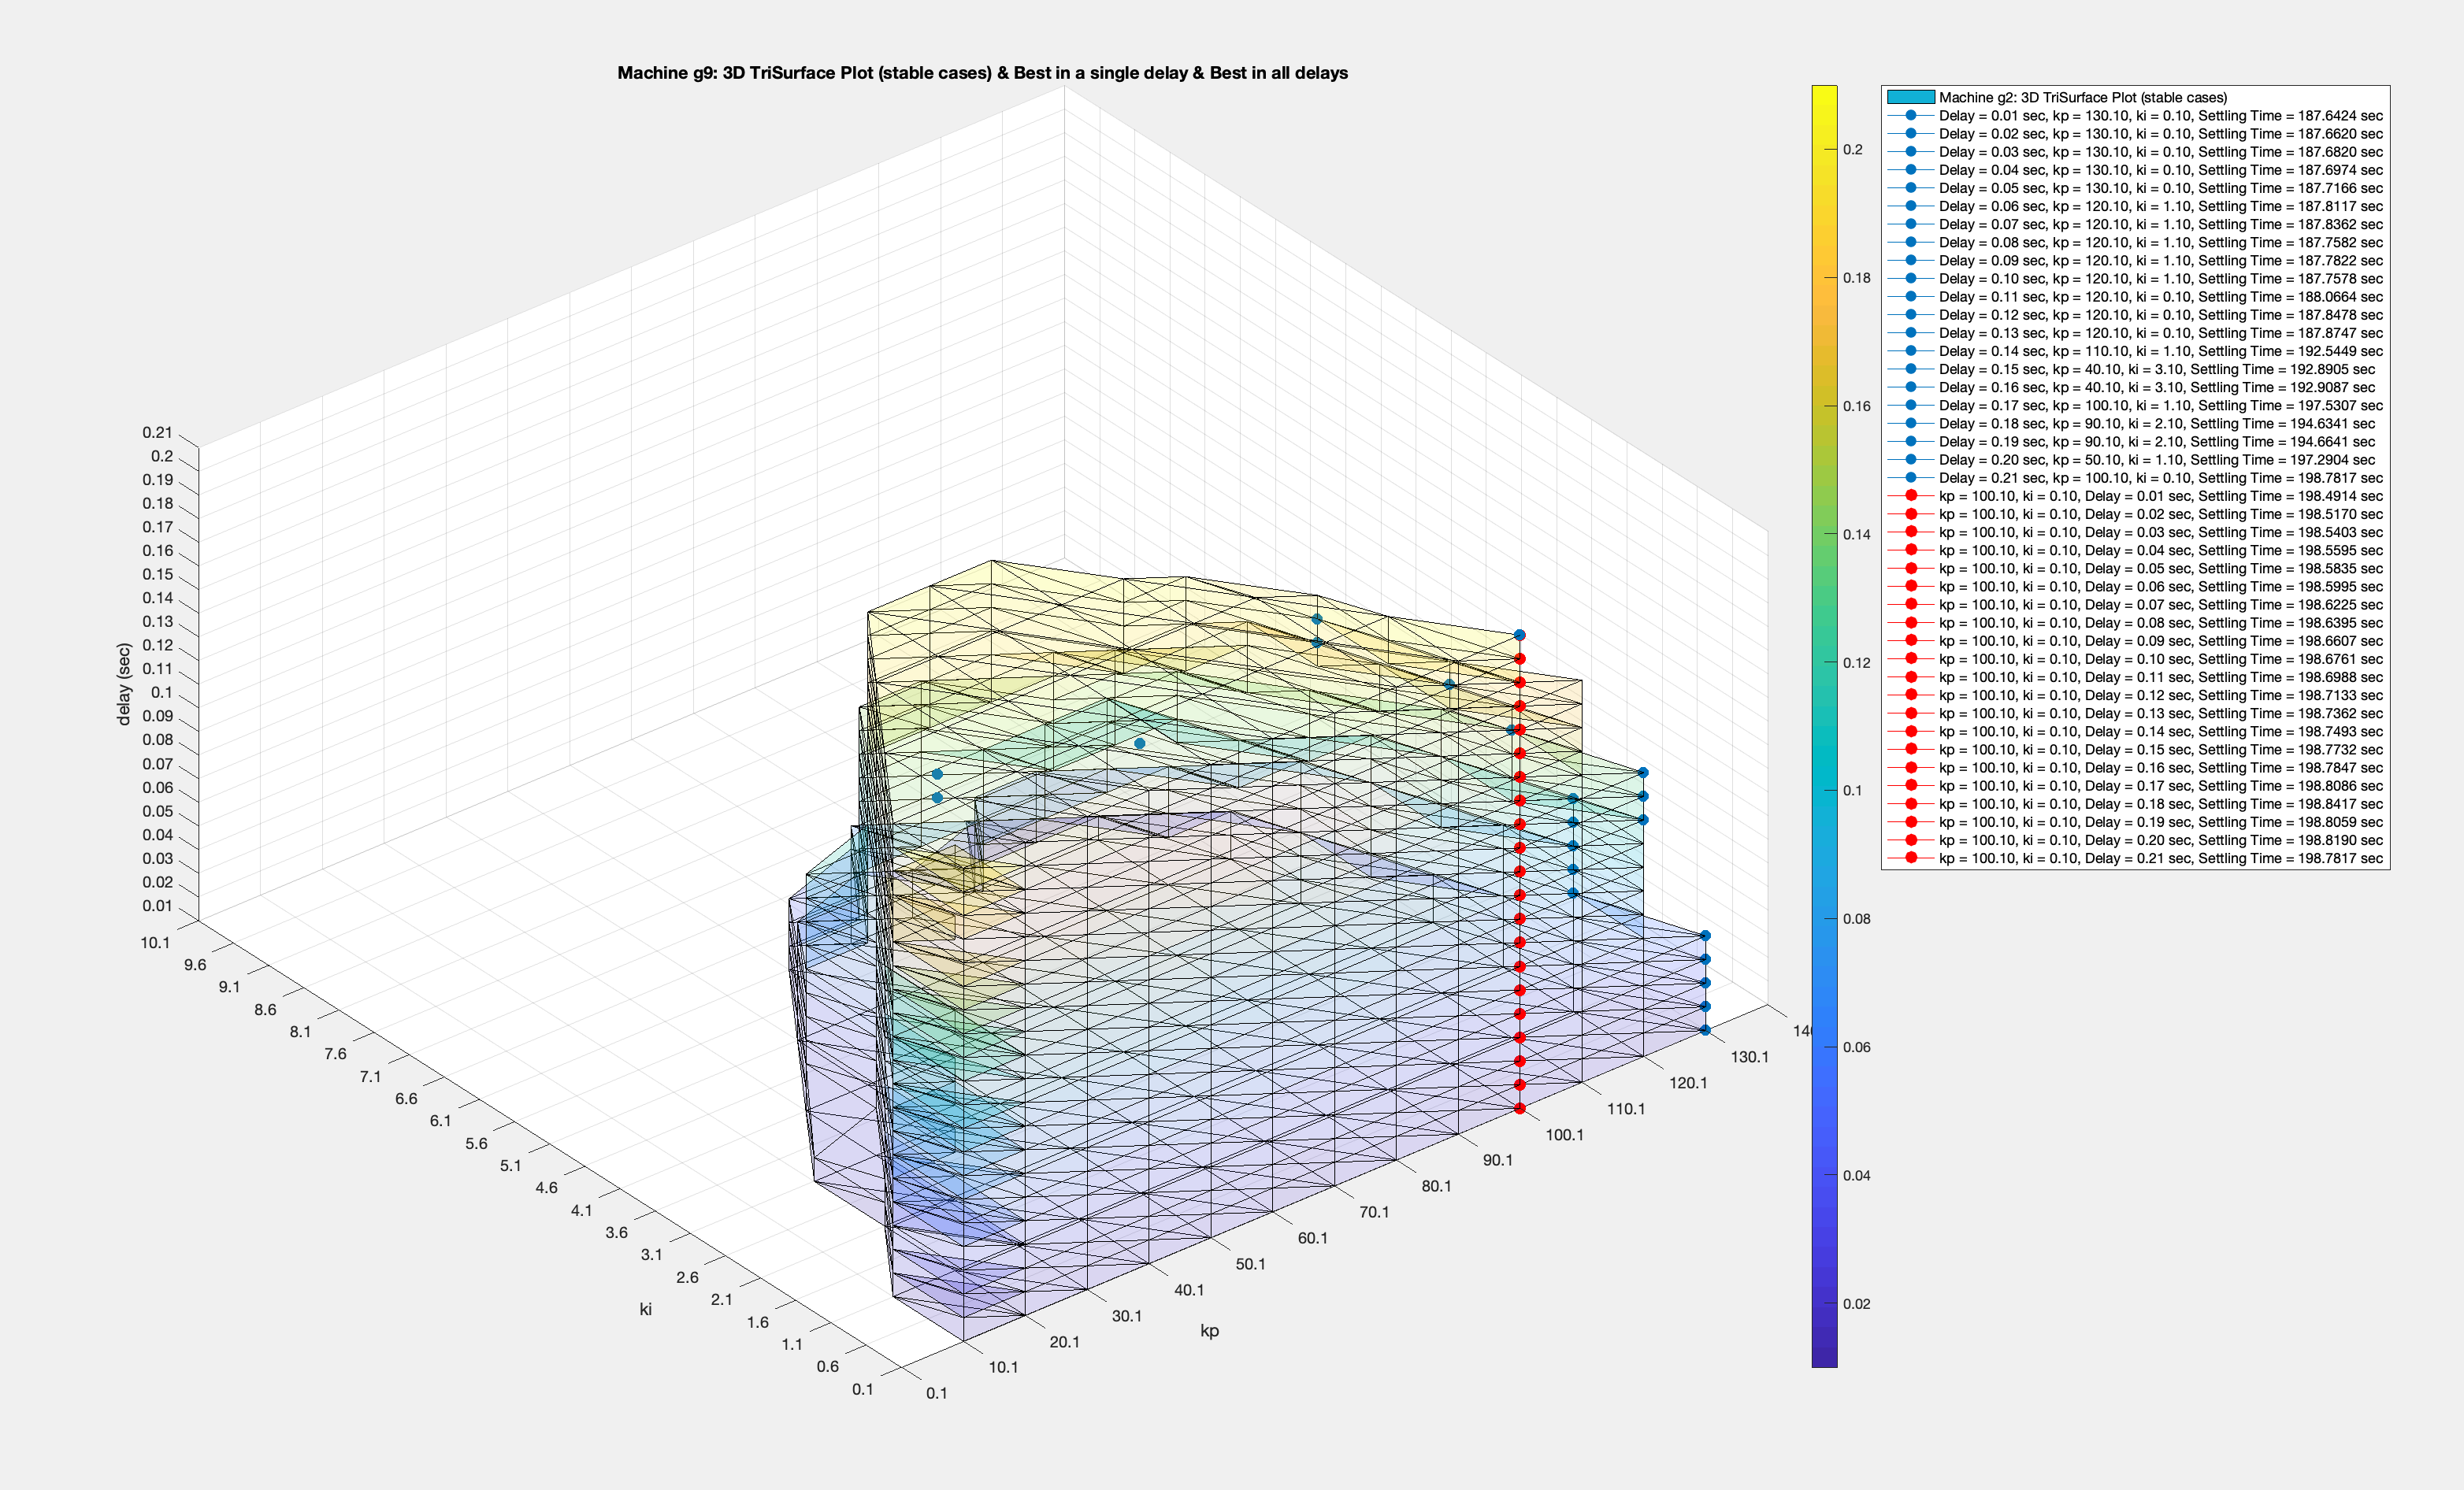
\includegraphics[width = .819\textwidth]{figure/5_4_1_without_Outlier4.png}
\caption{3D plot left side: without outliers}
\label{5_4_1_without_Outlier4}
\end{figure}


As we can see from Figure~\ref{5_4_1_without_Outlier1}, overall, the shape of the 3D plot shows kp and ki are shrunk together when the time delay increases. An increasing time delay removes some larger kis. Detailedly, if a controller has a larger kp and a large ki, the simulation results are recognised as unacceptable points in high probability. If a controller has a high kp but a small ki when the time delay is increased, the simulation results will not be recognised as unacceptable points in a large probability.\\

We rank the average settling time for every tuning situation. We finally find that when kp is 100.1 and ki is 0.1, the signal can approach fastest to the nominal value in average. 

Besides, we find that for the same ki and ki value, for instance, when kp is 100.1 and ki is 0.1, the settling time has a trend of increasing when time delay is increased. This directly prove the previous expectation on the impact of the time delay from Section~\ref{section5.2} and shows the time delay weakens the stability of the control.\\


Another important result is shown in the legend bar in the Figure~\ref{5_4_1_without_Outlier1}. The highlighted blue points are the best result for their delay. For example, “Delay = 0.01 sec, kp = 130.1, ki = 0.10, Settling Time = 187.6424sec” in the legend bar means when time delay is 0.01 seconds, the signal fastest approach to the nominal value if its kp is 130.1 and its ki is 0.10. We did not find that the kp value will increase if time delay increases as expected in Section~\ref{section5.2}. However, the reference of ki is changing: when delay is 0.01 seconds, the best ki is 0.01 however, when delay is 0.09 seconds, the best ki is 1.1, etc. The reason for this case might be the threshold for frequency (i.e. the frequency threshold should be in the range of 0.2\% in Nordic system) is too small for the signal. A large kp will first exceeds the limit of frequency threshold, then this large kp and its ki will have no chance appearing in the acceptable results.\\

\subsection{The Best Tuning Result} %5.4.2

The best tuning result is compared with the signal without SFC control and is shown in Figure~\ref{5_4_2}.

\begin{figure}[htbp]
\centering
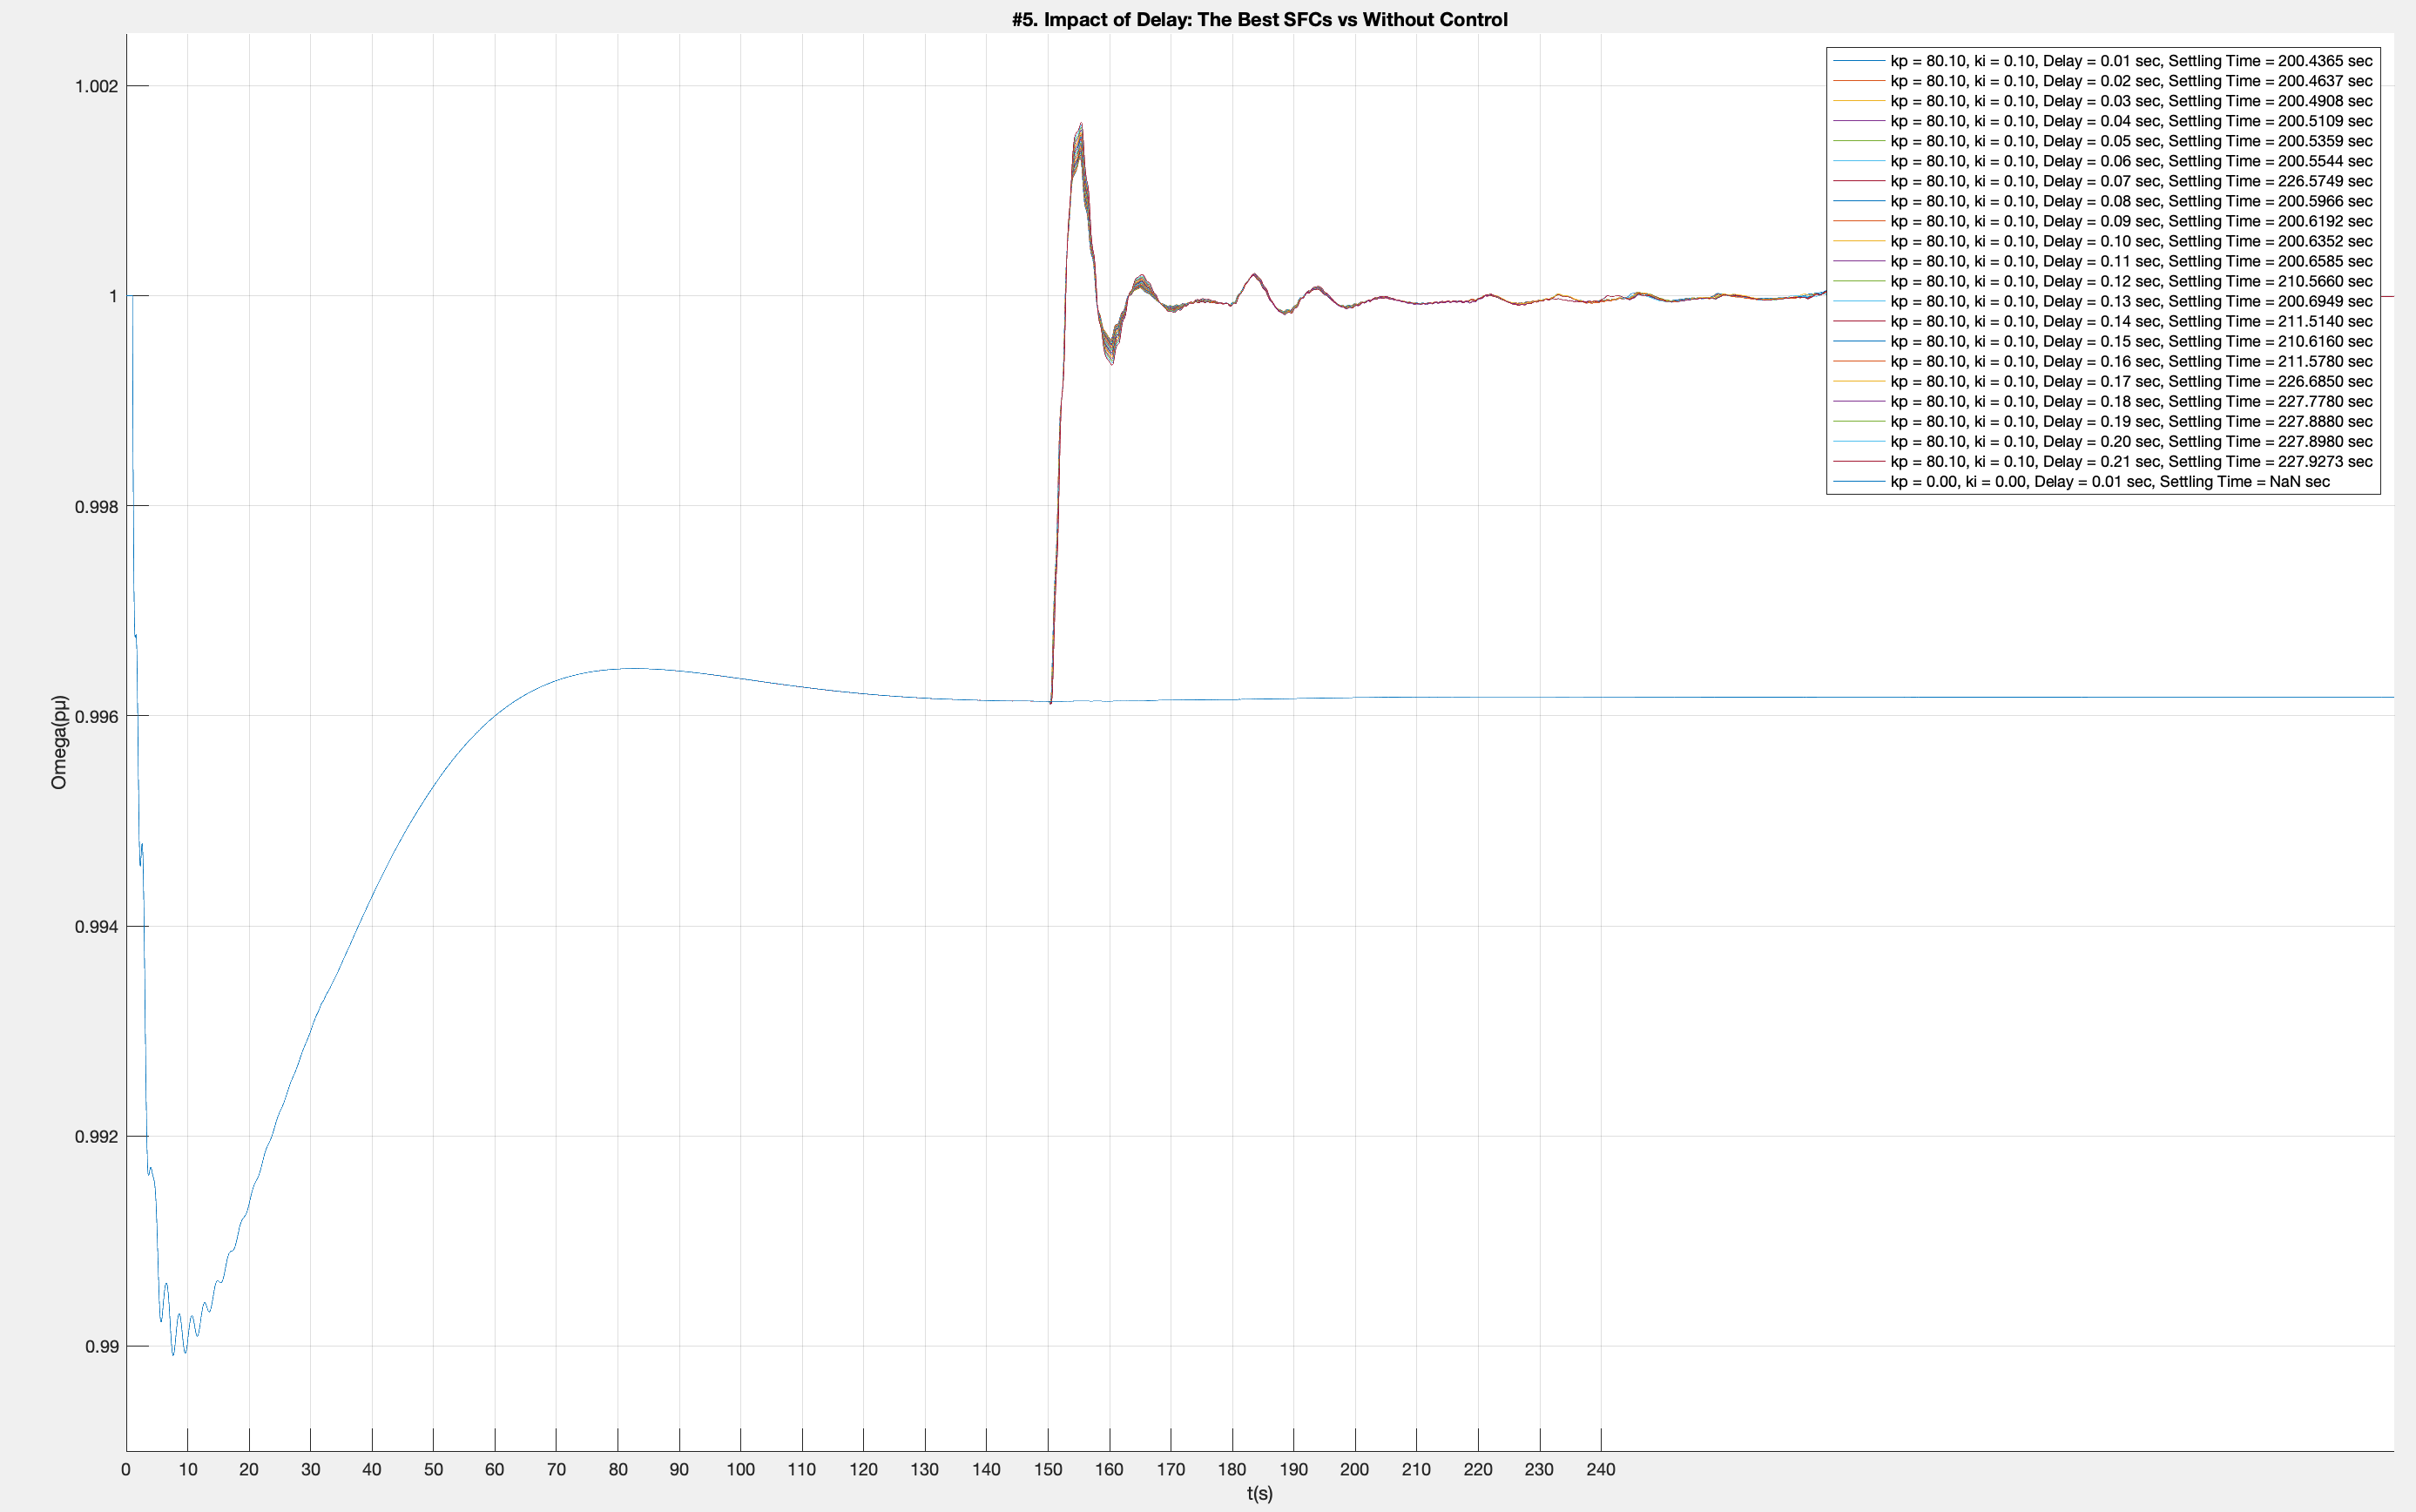
\includegraphics[width = .819\textwidth]{figure/5_4_2.png}
\caption{Impact of Delay: The Best SFCs vs Without Control}
\label{5_4_2}
\end{figure}